%==================================================================================================
%   LUKES THESIS TEMPLATE 1.2
%   -------------------------
%   This template is based upon the offcial IMM PhD Thesis template, it is enhanced with a number
%   of new features and a number of errors have fixed. This template is intended to be complied to
%   PDF using PDFLATEX and is tested using the MiKTeX 2.9 LaTeX distribution.
%   It is based on the official DTU-IMM Thesis template by Finn Kuno Christensen in 2009.
%   Small bugfixes by Kasper Laursen in 2012 and 2013.
%   -------------------------
%   Last Updated: 2012-09-19
%   Contact: lthhe@imm.dtu.dk
%==================================================================================================
%
%==================================================================================================
% DOCUMENT SETUP
%==================================================================================================
\documentclass[10pt,twoside,table]{book}                  %Official DTU-IMM Thesis document setup
%
%Set to 'print' for printed version, use 'net' for online version
\def\thesisversion{print}
%
%==================================================================================================
% PACKAGES
%==================================================================================================
\usepackage{LukeThesis}                            %Import Thesis base style
\usepackage{xcolor}
\usepackage{graphicx}
%\usepackage[utf8]{inputenc}
%\usepackage[T1]{fontenc}
%\usepackage{url}
\usepackage{xstring}
\usepackage{hyperref}
\usepackage{pdfpages}
\usepackage{placeins}
\usepackage[font=small,labelfont=bf]{caption}
\usepackage{subfig}

%\usepackage{subcaption}
\usepackage{enumerate}
\usepackage{amsmath}
\usepackage{listings} %for showing program code
\usepackage{bm}
\usepackage{wrapfig}
\usepackage{lipsum}
\usepackage{float}
\usepackage{titlesec}	
\usepackage{amsfonts}
\usepackage{amssymb}
\usepackage[square,authoryear]{natbib}
\usepackage{epstopdf}
\usepackage{tabularx}
\usepackage{siunitx}
\usepackage{mathtools}
\usepackage{tcolorbox}
\usepackage{lscape}
\usepackage{multirow}
\usepackage{setspace}
\usepackage{glslListings} 

\tcbuselibrary{breakable}

\newtcolorbox{mybox}{colback=red!3!white,colframe=red!75!black,breakable,arc=0pt,outer arc=0pt}

\bibpunct{[}{]}{,}{a}{,}{,}
\raggedbottom 
%\setlength{\parskip}{0pt}

%input{PhDMacros}                                   %Thesis specific macros
%
%==================================================================================================
% THESIS PROPERTIES (Modifiy these fields with your details)
%==================================================================================================
\def\thesisauthor{Alessandro Dal Corso}                     %Author
\def\thesistitle{Real-Time Rendering of Translucent Materials with Directional Subsurface Scattering}               %Title
\def\thesishandin{03-July}                       %Submission date (Day-Month}
\def\thesisdegree{M.Sc.}                              %Degree ('B.Eng', 'B.Sc.', 'M.Sc.' or 'PhD')
\def\thesisyear{2014}                               %Submission year
\def\thesisnumber{????}                             %DTU-IMM Serial number (do not include year)
\def\thesisISSN{0000-0000}                          %ISSN number
\def\thesiskeywords{subsurface,scattering,realtime,directional,dipole}  %PDF keywords
\derivethesisprops                                  %Derive dependent properties
%
%==================================================================================================
% SECTION NUMBERING SETUP
%==================================================================================================
\setcounter{tocdepth}{2}                            %2 adds sections up to subsections
\setcounter{secnumdepth}{3}                         %Subsubsections get a number when this is 3

\begin{document}
%------------------------
%Pre-frontmatter material
%------------------------
\prefrontmatter
%-------------------- 
%Frontmatter material
%--------------------
%\frontmatter
%\pagenumbering{roman}                               %Set frontmatter numbering style
%\chapter{Summary (English)}

The goal of the thesis is to ...                                   %English summary of Thesis
%\markboth{}{}                                       %Set headings (left)(right)
%\chapter{Summary (Danish)}
\begin{otherlanguage}{danish}

Målet for denne afhandling er at ...

\end{otherlanguage}                                   %Danish summary of Thesis
%\markboth{}{}                                       %Set headings (left)(right)
%\chapter{Preface}

\vspace{1cm}
This thesis was prepared at the DTU Compute department at the Technical University of Denmark in fulfillment of the requirements for acquiring an M.Sc. in Digital Media Engineering. 

The thesis deals with the efficient rendering of translucent materials, using an innovative model proposed by the author's M.Sc. thesis supervisor, Jeppe Revall Frisvad. Translucent materials consist of a particular class of materials like fruit, marble, skin, and other materials where subsurface scattering effects cannot be neglected. 

The interest for real time rendering in the author arose during the course of his M.Sc. in Digital Media Engineering, where he focused on the study line in Computer Games. For this study line, he had to take several courses in real time computer graphics, and from this courses he got his interest in advanced shading techniques. In the spring 2014, professor Jeppe Revall Frisvad of DTU Compute proposed a research-oriented M.Sc. thesis, that had the final goal of creating a method for implementing the directional dipole in real time. The author deemed the topic to be a great opportunity to research in real time rendering techniques, and so he registered his application for this master thesis, \emph{\thesistitle}.

The thesis consists of a software implementation in C++, Qt and OpenGL, and this report. The initial Qt framework used was taken from DTU course 02564, \emph{Real Time Graphics}, and then expanded in order to fit the needs of the thesis. All the code reported in this document was written by the author an does not come from the original framework. All the screenshots in this document were generated using the developed software. Other images in the report, unless the original source is reported in the caption, were generated by the author.

%==================================================================================================
% SIGNATURE AREA
%==================================================================================================
\begin{table}[ht]
\begin{tabularx}{\textwidth}{X}
\vspace{1.5cm}
Lyngby, \thesishandin-\thesisyear \\
\hfill \thesisauthor \\
\hfill 
\includegraphics[scale=0.4]{images/sig.png} \\
\end{tabularx}
\end{table}                                     %Preface
%\markboth{}{}                                       %Set headings (left)(right)
%\chapter{Acknowledgements}

I would like to thank my....

                            %Acknowledgements
%\markboth{}{}                                       %Set headings (left)(right)
%------------------
% Table of contents
%------------------
\newpage\mbox{}\newpage
\chaptermark{Contents}
\pdfbookmark{\contentsname}{toc}
\renewcommand{\sectionmark}[1]{\markright{#1}}
\sectionmark{Contents}
\addtolength{\parskip}{-\baselineskip}
\tableofcontents
\addtolength{\parskip}{\baselineskip}
\renewcommand{\sectionmark}[1]{\markright{\thesection\ #1}}
%-------------
% Main content
%------------- 
\mainmatter
\chapter{Introduction}
\label{chap:intro}
\emph{Subsurface scattering} (SS) is a physical phenomenon that naturally occurs in a wide range of natural materials. Some materials that exhibit a strong subsurface scattering effect in everyday life are milk, human skin and marble. Subsurface scattering occurs when light is partially absorbed by an medium, bounces repeatedly inside ("scatters") and finally exits the surface on another point of the material (as in Figure \ref{fig:ssdiagram}). The phenomenon that results is generally known as \emph{translucency}. We can see some examples of translucent objects in Figure \ref{fig:ex1}.

\section{Background}
Since the beginning of computer graphics, various attempts have been performed in order to model subsurface scattering. Some of these models involve Monte Carlo simulations of the light entering the medium \citep{Pharr:2000:MCE:344779.344824}, or other numerical techniques \cite{Fattal:2009:PMI:1477926.1477933,Kaplanyan:2010:CLP:1730804.1730821}. Other focus on approximating the diffusion of light within the material using an analytical approach, like \citep{Jensen:2001:PMS:383259.383319}.
 
\clearpage
\begin{figure}[!ht]
\centering
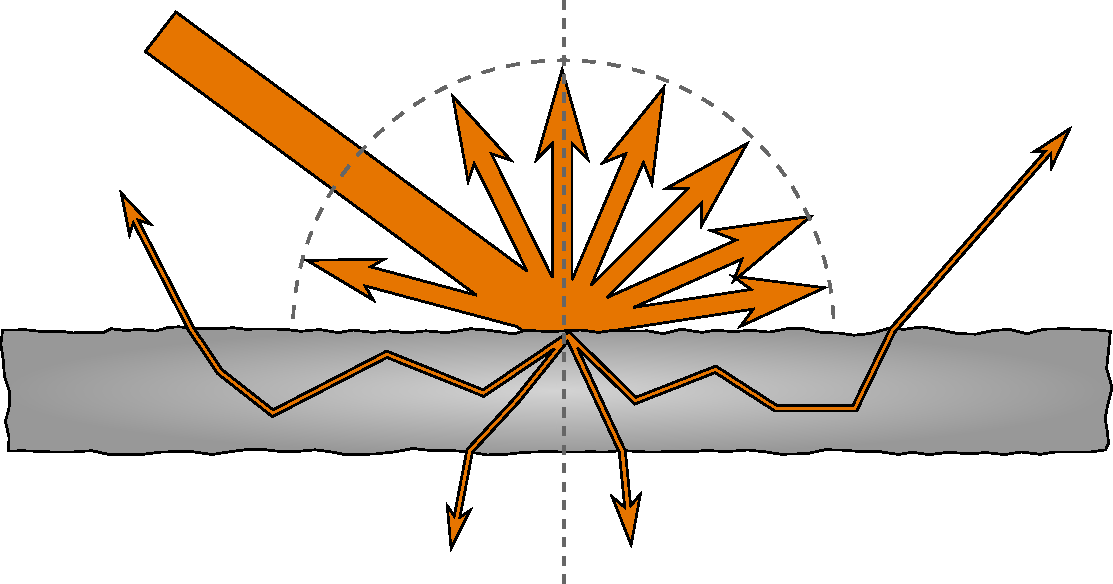
\includegraphics[width=0.8\textwidth]{images/diagram.pdf}
\caption{Diagram of subsurface scattering. Most of the incoming light gets reflected, but some of it enters the material and leaves it at a different point.}
\label{fig:ssdiagram}
\end{figure}

The first model that proposed an analytical approach was the one by \cite{Jensen:2001:PMS:383259.383319}, as an approximation of the radiative transfer equation. This approximation, called the \emph{diffusion approximation} \citep{books/daglib/0093591} has been exploited by different authors, in order to account for multi-layered materials \citep{Donner:2005:LDM:1186822.1073308}, heterogeneous materials \citep{journals/cgf/WangWHSYG10} and thin surfaces\citep{journals/cgf/WangWHSYG10}. A recent analytical model, proposed by \cite{IMM2013-06646}, extends the approximation in order to account for the directionality of the incoming light. All these analytical methods are based on BSSRDF models. A BSSRDF function is a functions that describes how light is transmitted between two points in a material, and is a generally dependent on the incoming light direction, the distance between the two points and the outgoing light direction.

In recent years, with the advent of programmable graphics cards (GPU), it has become possible to exploit these algorithms and bring them to interactive frame rates, and in some cases even to real time rendering. \cite{Jensen:2002:RHR:566654.566619} were the first to propose an efficient implementation for rendering subsurface scattering using an octree. More recently, several methods have been proposed, including image-based splats \citep{4736459}, sum-of-Gaussians filtering \citep{d'Eon:2007:ERH:2383847.2383869}, and grid-propagation based methods \citep{Borlum:2011:SSL:2018323.2018325}. We will introduce in detail some of these methods in Chapter \ref{chap:previous}, were we will review the existing literature in more detail.

\begin{figure}
\centering
\subfloat{
  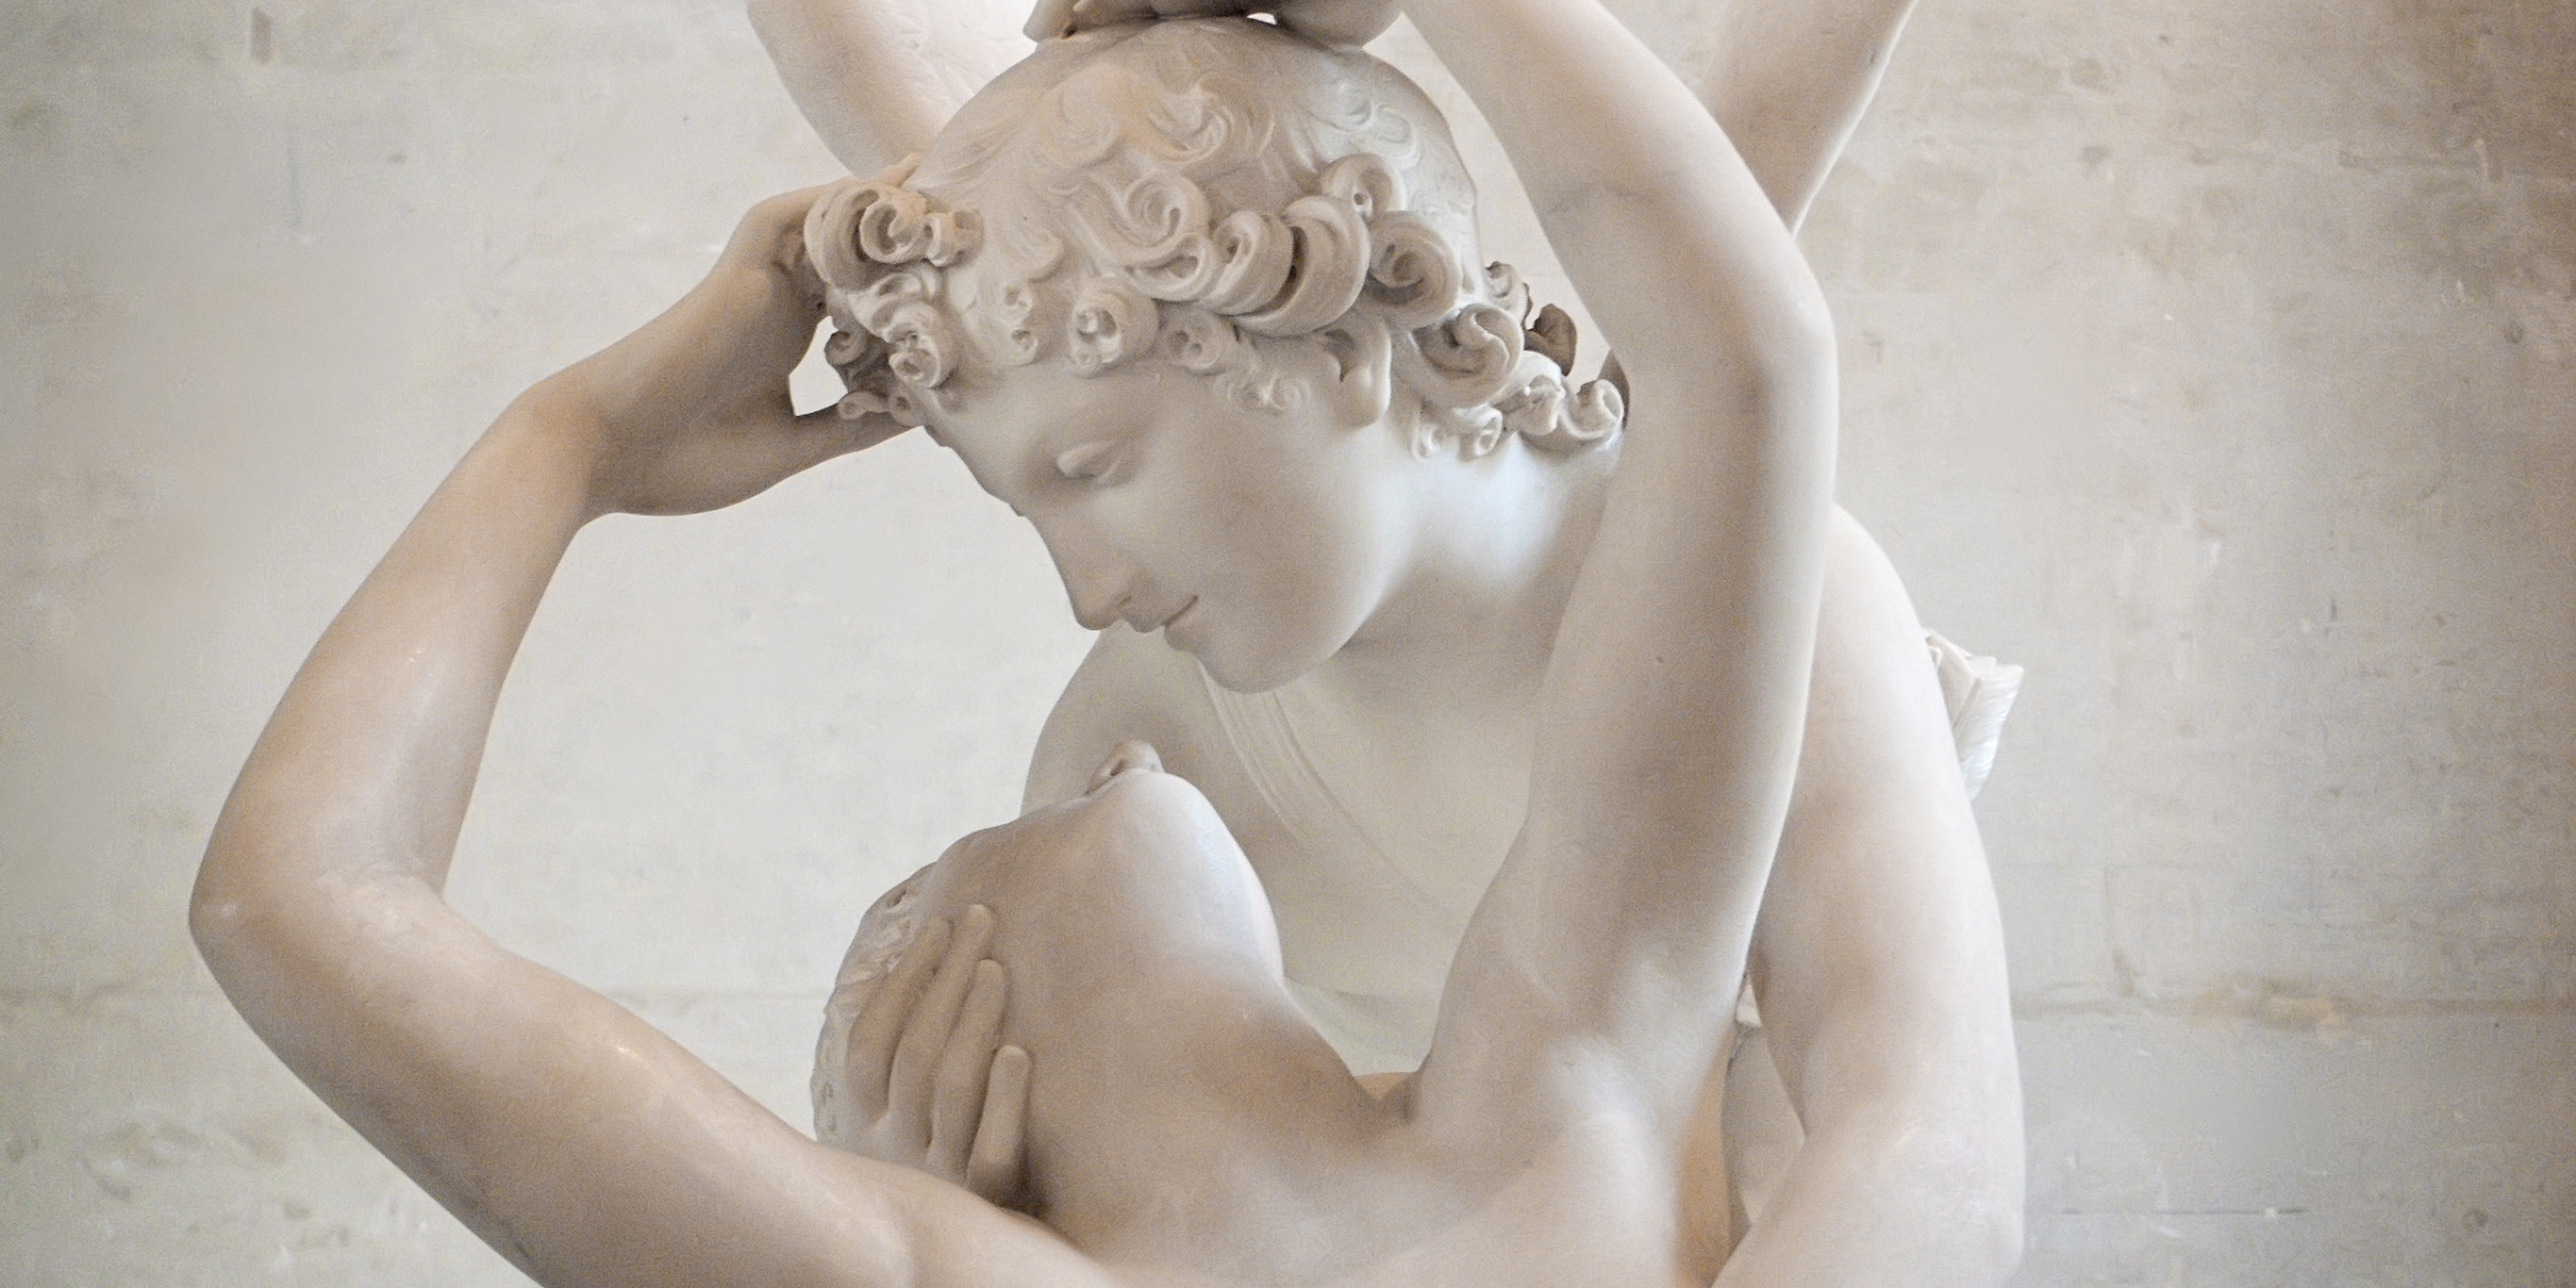
\includegraphics[width= 0.9 \linewidth]{images/marble.jpg}
  \label{fig:ss1}
}
\\
\subfloat{
  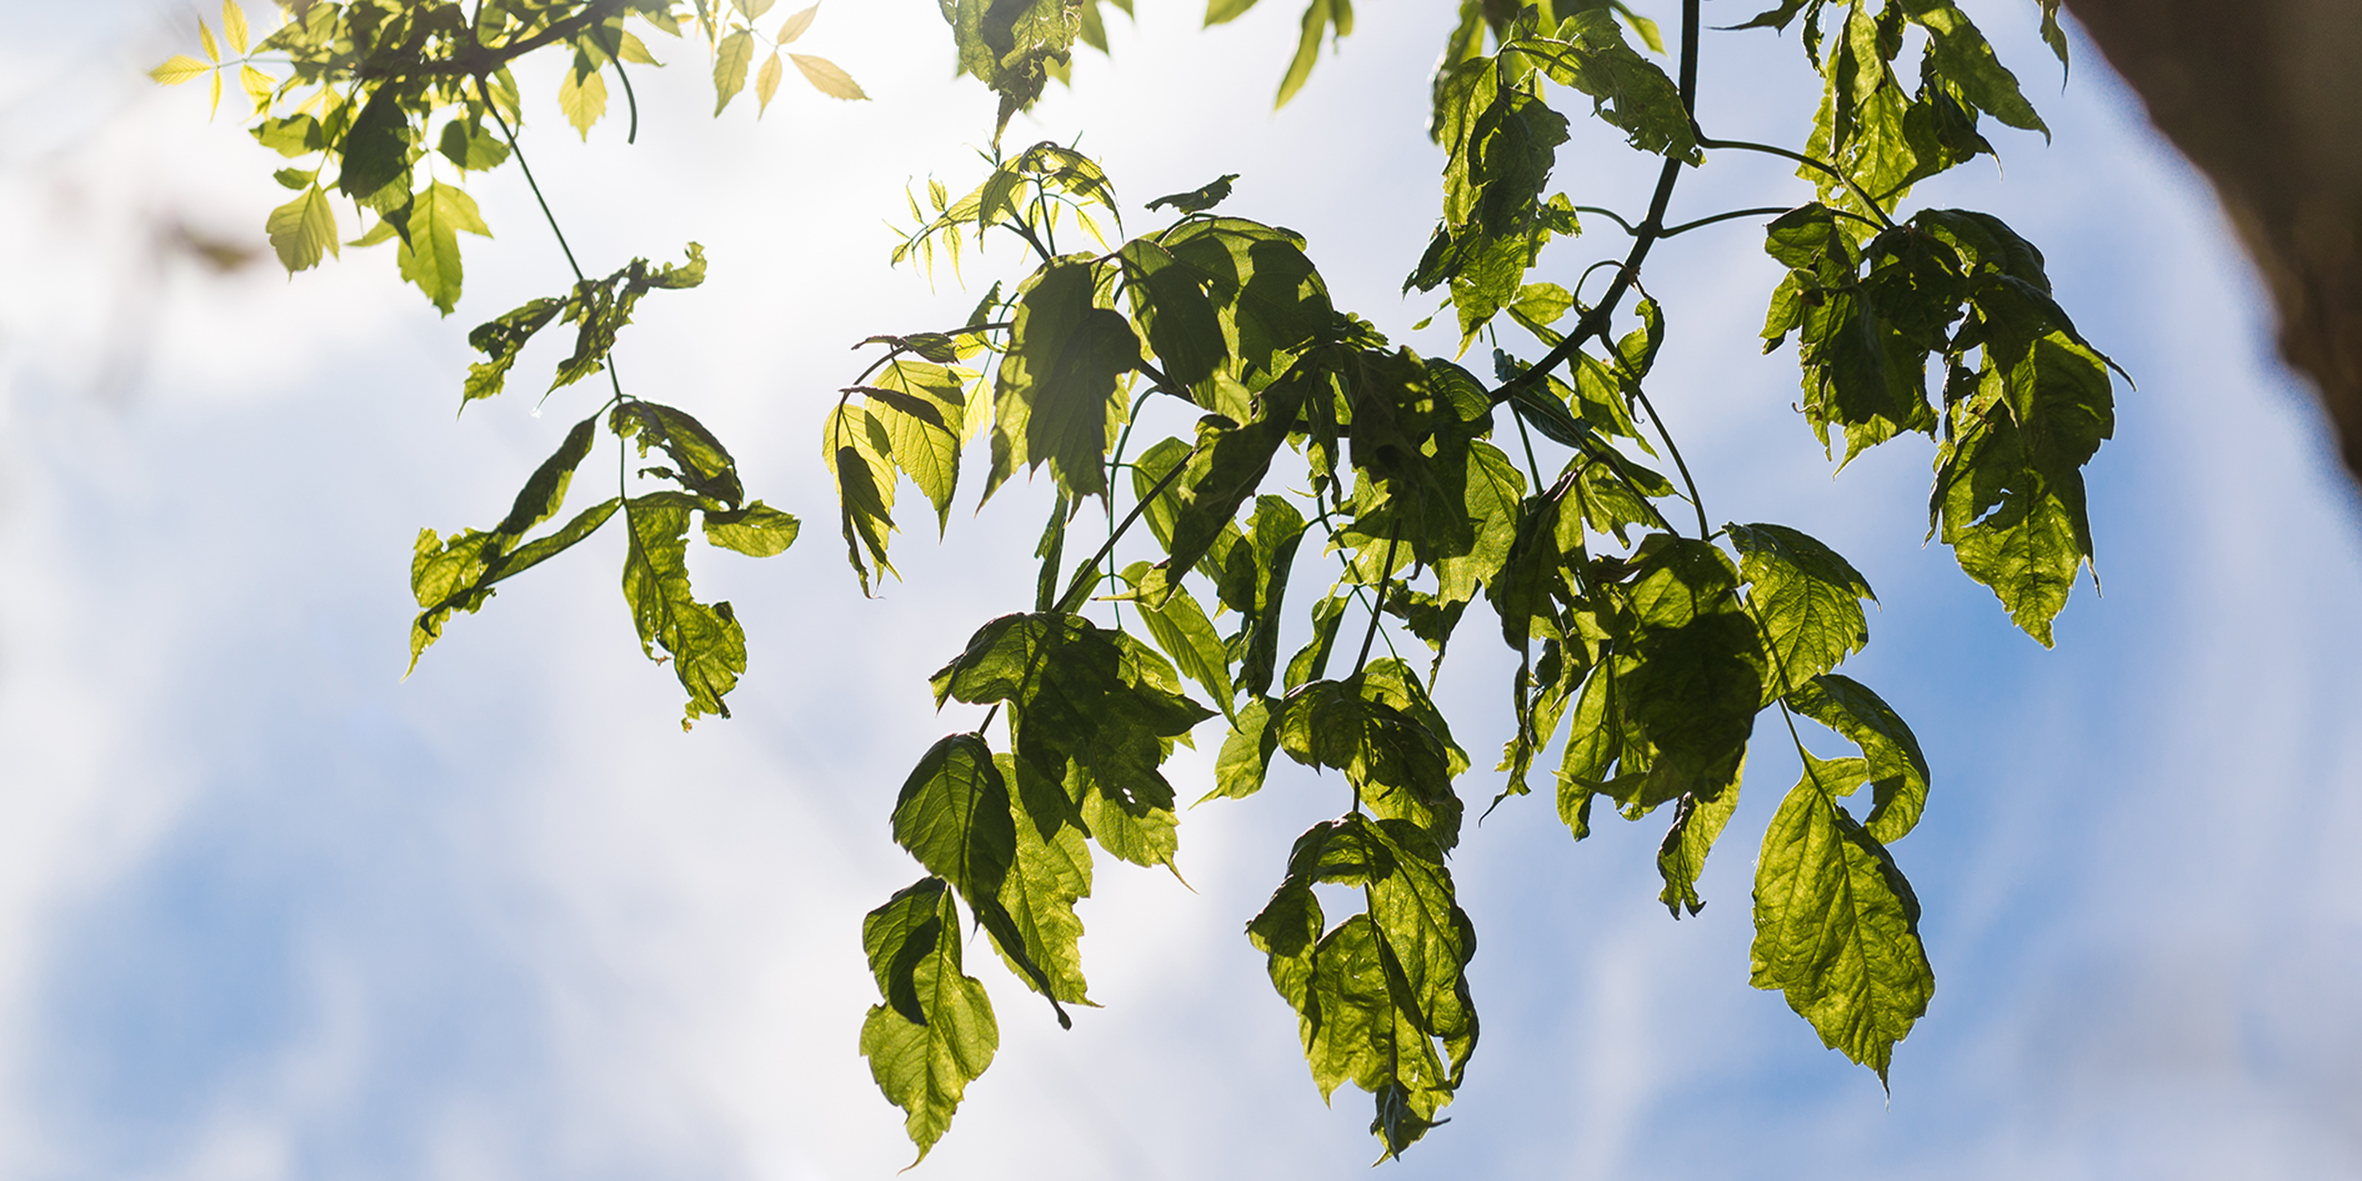
\includegraphics[width= 0.9 \linewidth]{images/leaves.jpg}
  \label{fig:ss2}
} 
\\
\subfloat{
  
\includegraphics[width=0.9 \linewidth]{images/candle.jpg}
  \label{fig:ss3}
} 
\caption{Some examples of translucent materials: marble, leaves and wax. The marble image and the candle are under the \href{http://creativecommons.org/licenses/by-sa/2.0/deed.en}{cc-by-sa} license, and are courtesy of Wikimedia Commons. The two images were cropped to fit the document. The leaves image was taken by Alberto Bedin and is used with permission.}
\label{fig:ex1}
\end{figure}

\section{Problem statement}

The goal of this thesis is to implement a real-time rendering technique in order to render directional subsurface scattering using the analytical model proposed by \cite{IMM2013-06646}. The technique should ideally obtain the same results as a offline rendered solution of the original model, but reducing the rendering times to a few milliseconds. To do this, we employ the aid of the GPU programmable pipeline \citep{Fernando:2004:GGP:983868}. 

We found that there is a current gap in the knowledge on current real-time subsurface scattering techniques regarding the approach to directional models. In fact, most of the methods rely on the assumption that the BSSRDF function depends only on the distance between the entering and exiting point \cite{Jensen:2001:PMS:383259.383319}. This allows, for example, to pre-compute the BSSRDF function and use it in the computations, greatly increasing the performance \citep{4736459}. However, in the model proposed by \cite{IMM2013-06646}, this is not possible, as the direction of the incoming light must be taken into account. In fact, the model has too many degrees of freedom to make a pre-computation feasible. 

The model proposed by \cite{IMM2013-06646} offers a more realistic evaluation of subsurface scattering effects. A real-time working implementation would improve the quality of scattering materials in real-time graphics applications, such as real-time architectural visualization and computer games. In the latter field, in recent years there has been a renewed interest in real-time SS techniques, especially to model faithfully the appearance of skin on human faces. 

\section{Requirement analysis}

In this section, we will introduce some constraints and assumptions to limit the scope of our work. Some of these assumptions and constraints are well known to the graphics community, and they are generally introduced to allow better performance, quality and flexibility. Being a real-time rendering method implies that performance plays a big part in the decisions we have made in the process, but since the method uses a physically based approximation the final quality of the result is also important. In the process the aspect of flexibility has been taken into account, i.e. the capacity of the method to set the tradeoff between quality and performance. We will now list the assumptions we made in all the three described domains, quality, performance and flexibility. 

\subsection{Quality constraints}
 \label{sec:quality}
\begin{enumerate}
\setlength{\itemsep}{-1pt}
	\item Be visually close as much as possible to a offline rendered solution.
	\item Be consistent with the directional dipole model for a wide range of material properties. In particular, the method should perform well in the domain of quality where the directional dipole model excels (highly scattering materials).
	\item Be potentially able to render an object under an arbitrary number of different types of lights (point, directional, environment, etc.).
\end{enumerate}

\subsection{Flexibility requirements}	
\begin{enumerate}
\setlength{\itemsep}{-1pt}
	\item Work with the less amount as possible of provided model data, i.e. only the position data and eventually the normals should be provided in order for the method to run. In particular, no unwrap of the mesh (UV mapping) should be necessary. 
	\item Being able to be integrated in a game engine environment, using data from other computations (e.g. other lighting computations) and being adaptable to different lighting paths (forward and deferred shading).
  \item The quality versus performance tradeoff should be set by a potential artist or developer, with the fewest number of parameters as possible.
\end{enumerate}

\subsection{Performance requirements}
\begin{enumerate}
\setlength{\itemsep}{-1pt}
	\item Being real-time on a high-end modern GPU, i.e. one frame should take less that 100 ms (10 FPS) to render. The ideal result would be to reach a rendering time of less than 16 ms (60 FPS).
	\item Being as less dependent as possible from the geometrical complexity of the model.
	\item Being as less dependent as possible from the screen resolution.
	\item If the desired quality is not reachable within one frame, converge towards a result in a reasonable amount of time. Techniques should be used to approximate the required quality for the intermediate result. 
	\item Maintain a reasonable performance under changing light conditions, deformations and change of parameters, with little or none performance penalties.
	\item Employ the advantages of the directional dipole model to improve performance.
	\item Support up to a certain number of directional and point lights (up to 3 to 5 pixel lights, as in commercial engines\citep{unitymanual}).
	\item Require little or no pre-processing in order to be able to perform. If there is any pre-processing involved, it should be performed only at the beginning of the life cycle of the program. 
\end{enumerate}

%\section{Method overview}
%
%Our method consists of introducing the assumption that only the points within a certain radius from the point are contributing to the exiting light. Then, we take a certain number $N$ of these surface samples and compute their contribution to calculate the exiting light. The samples are distributed with an exponential distribution, in order to account more for the samples closest to the exiting point. The reader can get more details on the method in Chapter \ref{chap:method}. 

\section{Thesis Outline}
In this Chapter, we have given an introduction to the problem and stated the assumption that will guide us through the choices that we will make through our thesis. In Chapter \ref{chap:previous}, Related Work, we will describe in more detail some of the different approaches to subsurface scattering in literature. In Chapter \ref{chap:theory}, we will give a theoretical introduction to subsurface scattering and light transport theory, with a special focus on BSSRDF functions. In Chapter \ref{chap:method}, we will describe our method on approaching the problem on a theoretical basis. In Chapter \ref{chap:implementation} we will describe the actual implementation of the method, and the problems and limitations met during the process. In Chapter \ref{chap:results}, we will describe the tests we made and show the results, both in the domain of performance and quality, comparing them with the requirement analysis we made in the previous section. Then, we will describe some possible extensions to the method in Chapter \ref{chap:futurework}. We will wrap up everything in Chapter \ref{chap:conclusions}, where we will give our conclusions. 
\clearpage
\chapter{Related Work}
\label{chap:previous}
In rendering of subsurface scattering, most approaches rely on approximating correctly the \emph{Radiative Transfer Equation} (RTE). We identified two main approaches to the problem in literature:

\begin{description}
	\item[Analytical] One class of solutions consists of approximating the RTE or one of its approximations via an analytical model. These models can have different levels of complexity and computation times, and are often adaptable to a wide range of materials. However, often they rely on assumptions on the scattering parameters that limit their applicability.
	\item[Numerical] In this other class of solutions, a numerical approach is used instead of approximating the RTE with an analytical model. This methods include finite element methods and discrete ordinate methods, for which a numerical solution for the RTE is actually computed. While providing an exact solution, the computation times are longer. Other numerical approaches focus more on the appearance of the model and do not provide an exact solution for the RTE.
\end{description}

In this thesis, we focus on efficiently implementing a model that falls in the first category, the analytical models. In the following sections, we are going to describe approaches for each one of the mentioned categories, comparing them to our method.

\section{Analytical techniques}

In the analytical techniques, two different areas of research must be distinguished. The first area is the research on the actual models, while the second is research on how the actual models can be implemented efficiently. Each model is usually represented by a specific function called BSSRDF (\emph{Bidirectional Subsurface Scattering Reflectance Distribution Function}), that describes how light propagates between two points on the surface. Two integrations, one on the surface one from all the directions, must be performed in order to get the amount of light that actually exits from a point on the surface (see chapter \ref{chap:theory}). Implementation techniques focus on efficiently implementing this integration steps, often making assumptions for which points computations can be avoided. 

\subsection{Models}
Regarding the models, the first and most important is the dipole developed by \cite{Jensen:2001:PMS:383259.383319}. This models relies on an approximation of the RTE called the \emph{diffusion approximation}, which again relies on the assumption of highly scattering materials. In this case, a BSSRDF for a planar surface in a semi-infinite medium can be obtained. The BSSRDF needs only the distance between two points to be calculated, and with some precautions can be also used with arbitrary geometry. This model does not include any single scattering term: it needs to be evaluated separately. The model has been further extended in order to account for thin object regions and multi-layered materials \citep{Donner:2005:LDM:1186822.1073308}.

A significant improvement of the model was later given by \cite{deondeon}, that improved the model to better fit path traced simulations without nearly any additional computation cost. A more advanced model based on quantization was proposed by \cite{D'Eon:2011:QMR:1964921.1964951}, that introduced a new physical foundation in order to improve the accuracy of the original diffusion approximation. Finally, some higher order approximation exist \citep{PhysRevLett.94.153904, IMM2013-06646}, in order to account for the directionality of the incoming light and single scattering. This allows a more faithful representation of the model at the price of extended computation times. A comparison between the directional and the standard dipole can be seen in figure \ref{fig:bssrdfcomparison}.


\subsection{Implementations}

Most research on efficient implementations of a subsurface scattering analytical model has been made on the original model by \cite{Jensen:2001:PMS:383259.383319}. The first efficient implementation was proposed by \cite{Jensen:2002:RHR:566654.566619}, based on a two-pass hierarchical integration approach. Samples on the model are organized in an octree data structure, that then is used to render the object. In the first step, the radiance from the light is stored in the points. In the second pass, using the octree, the contribution from neighboring points is computed, clustering far points in order to speed up calculations. This approach can be adopted for the Jensen model, where the only parameter is the distance between the entering and exiting point. However, using the directional dipole, the samples cannot be clustered because of the directionality of the light: once we sum up the contribution from multiple lights, the contribution cannot be separated anymore. In fact, we would need a different clustering of the points for each light, that quickly becomes inefficient since whole octree would have to be stored on the GPU. 

\cite{Lensch:2002:IRT:826030.826632} approached the problem by subdividing the subsurface scattering contribution into two: a direct illumination part and a global illumination part (i.e. the light shining through the object). The global illumination part is pre-computed as vertex-to-vertex throughput and then summed to the direct illumination term in real-time. Compared to our method, this method requires a pre-computation step that depends on the geometry of the model, and thus deformation effects are not possible. Moreover, a coefficient has to be stored for each pair of vertex, that means a quadratic increase for increasing model size. Our method, on the other hand, occupies a memory space depending linearly on the number of vertices.

Translucent shadow maps \citep{Dachsbacher:2003:TSM:882404.882433} use an approach similar to standard shadow maps: they render the scene from the light point of view, and then calculate the dipole contribution in one point only from a selected set of points, according to a specified sampling pattern. As in \cite{Lensch:2002:IRT:826030.826632}, the contribution is split into global and local to permit faster computations. In our approach we will reuse some of the ideas introduced by translucent shadow maps: we will render the scene from the light point of view and we will reuse the information stored in the map such as depth, vertices and normals. However, our approach to using the values from the map is different from the original paper, as we will explain in chapter \ref{chap:method}. \cite{Mertens:2003:IRT:882404.882423} propose a fast technique based on radiosity hierarchical integration techniques, that unlike the previous implementation can handle deformable geometry.

Another important category of methods is screen space methods. \cite{1238246} propose an image space GPU technique that pre-computes a set of sample points for the area integration and then performs the integral over multiple GPU passes. \cite{d'Eon:2007:ERH:2383847.2383869,deonss} propose a method in image-space, interpreting subsurface scattering as a sum of images to which a gaussian filter has been applied. The gaussians are then summed with weights that make them fit the diffusion approximation. \cite{Jimenez:2009:SPR:1609967.1609970} improves further the technique, giving more precise results in case of skin. All these techniques assume that the diffusion profile can be pre-computed and then fitted with a sum of Gaussians: as we have already mentioned, this is not possible for the directional dipole, where the diffusion profile can change a lot depending on the angle of incidence of the incoming ray of light. Moreover, even if we were able to compute the coefficients for each possible combination of parameters, it would not be possible to apply a gaussian filter with a different set of coefficients per point.

\cite{4736459} present a fast screen space technique that render the object as a series of splats, using GPU blending to sum over the various contributions. The diffusion profile in this case is pre-computed and stored as a texture. As in the previous techniques, the directionality of the incoming light does not allow the pre-computation of a diffusion profile. Moreover, the directional dipole is not symmetrical, so the splats would have to use a bigger radius in order to account for all the contribution, increasing computation costs.

\section{Numerical techniques}

Numerical techniques for subsurface scattering are often not specific, but come for free or as an extension of a global illumination numerical approximation, since the governing equations are essentially the same. Given their generality, they are usually slower than their analytical counterpart, and often rely on heavy pre-computation steps in order to achieve interactive framerates. The volumetric version of Jensen's Photon Mapping\citep{Jensen:1998:ESL:280814.280925} was originally developed to render participating media in general, but it has been adapted for subsurface scattering\citep{Dorsey:1999:MRW:311535.311560}. Classical approaches as a full Monte-Carlo simulation implementation of the light-material interaction, and finite-difference methods exist in literature\citep{raey}. 

Some less general methods have been introduced in order to devise more efficient approximations when it comes to the specific problem of subsurface scattering. \cite{raey} uses the diffusion approximation with the finite difference method on the object discretized on a 3D grid. \cite{Fattal:2009:PMI:1477926.1477933} uses as well a 3D grid, that is swept with a structure called light propagation map, that stores the intermediate results until the simulation is complete. All the numerical methods described so far are not real-time, and they are generally not feasible for a GPU environment. 

\cite{journals/cgf/WangWHSYG10}, instead of performing the simulation on a discretized 3D grid, makes the propagation directly in the mesh, converting it into a connected grid of tetrahedrons called \emph{QuadGraph}. This grid can be optimized to be GPU cache friendly, and provide a real-time rendering of deformable heterogeneous objects. The problem in this method is that the QuadGraph is slow to compute (20 minutes for very complex meshes) and has heavy memory requirements for the GPU. Compared to our method, this one requires an heavy pre-computation step, and allows only not-deformable objects. However, as most of propagation techniques, it can handle heterogeneous materials, while our method can not.

Precomputed radiance transfer methods are another class of general global illumination methods, that generally pre-compute part of the lighting and store it in tables\citep{Donner:2009:EBM:1531326.1531336}, allowing to retrieve it efficiently with an additional memory cost. The problem with this method compared to ours is that it requires a memory space that increases exponentially if we want to handle deformable materials and dynamic lighting. Moreover, it requires an heavy pre-computation in order to calculate the lighting coefficients. Our method, being analytical, does not required either a lot of memory or an heavy pre-computation step. 

A recent method called SSLPV (\emph{Subsurface Scattering Light Propagation Volumes}) \citep{Borlum:2011:SSL:2018323.2018325} extends a technique originally developed by \cite{Kaplanyan:2010:CLP:1730804.1730821} to propagate light efficiently in a scene using a set of discretized directions on a 3D grid. The method allows real-time execution times and deformable meshes with no added pre-computation step, with the drawback of not being physically accurate. Moreover, the required memory space on the GPU is larger than the one required than our method, since a voxelization of a mesh must be stored. 

Finally, for real-time critical applications (such as games), translucency is often estimated as a function of the thickness of the material, that is used to modify a lambertian term \citep{Tomaszewska2012,greenrtss}. A method by \cite{Kosaka:2012:RAR:2407156.2407206} uses an approach similar to the one we will describe in order to compute the thickness of the material using a different camera direction. While not physically accurate, this techniques allows to have a fast translucency effect that can be easily added to existing deferred pipelines. Compared to our method, this method requires no storage space and light computation. However, the risk is that the translucency effects are not represented faithfully, and some artifacts may appear, as pointed out in \cite{greenrtss}, and multi-sampling should be used in order to avoid artifacts. 

As we can see, in the reviewed literature so far there is not a proper way to account for direction in subsurface scattering in real-time, or at least one that satisfies the requirements we have made in chapter \ref{chap:intro}. We will introduce in detail our method to handle directional subsurface scattering in real-time in chapter \ref{chap:method}. In the next chapter, we are going to give a theoretical introduction to a mathematical description of light transport, as well as giving the proper formulas and definition of the standard dipole model by \cite{Jensen:2001:PMS:383259.383319} and the directional dipole model presented by \cite{IMM2013-06646}. 


\appendix
\chapter{Model matrices}
\renewcommand{\arraystretch}{1}
\label{sec:matrices}
\section{Model matrices}

\textbf{Translation matrix}

$$T(\mathbf{t}) = \left[\begin{array}{cccc}
1 & 0 & 0 & \mathbf{t}_x       \\
0 & 1 & 0 & \mathbf{t}_y       \\
0 & 0 & 1 & \mathbf{t}_z       \\
0 & 0 & 0 & 1
\end{array}\right]$$


\textbf{Rotation matrix}

$$R_x(\theta) = \left[\begin{array}{cccc}
1 & 0 & 0 & 0       \\
0 & \cos\theta & -\sin\theta & 0       \\
0 & \sin\theta & \cos\theta & 0      \\
0 & 0 & 0 & 1
\end{array}\right]$$

$$R_y(\theta) = \left[\begin{array}{cccc}
\cos\theta & 0 & \sin\theta & 0       \\
0 & 1 & 0 & 0       \\
-\sin\theta & 0 & \cos\theta & 0      \\
0 & 0 & 0 & 1
\end{array}\right]$$

$$R_z(\theta) = \left[\begin{array}{cccc}
\cos\theta & -\sin\theta & 0 & 0       \\
\sin\theta & \cos\theta & 0 & 0       \\
0 & 0 & 1 & 0      \\
0 & 0 & 0 & 1
\end{array}\right]$$

\textbf{Scale matrix}

$$S(\mathbf{s}) = \left[\begin{array}{cccc}
\mathbf{s}_x & 0 & 0 & 0       \\
0 & \mathbf{s}_y & 0 & 0       \\
0 & 0 & \mathbf{s}_z & 0      \\
0 & 0 & 0 & 1
\end{array}\right]$$

\section{View Matrix}

$\mathbf{e}$ is the camera position, $\mathbf{d}$ is the camera direction, $\mathbf{u}$ is the up vector.

\begin{equation*}
\begin{split}
\vec{c} &= -\frac{\mathbf{d}}{\|\mathbf{d}\|} \\
\vec{a} &= \frac{\vec{c} \times \mathbf{u}}{\|\vec{c} \times \mathbf{u}\|} \\
\vec{b} &= \vec{a} \times \vec{c} 
\end{split}
\end{equation*}

$$
V(\mathbf{e},\mathbf{d},\mathbf{u}) = \left[\begin{array}{cccc}
\vec{a}_x & \vec{a}_y & \vec{a}_z & -\mathbf{e}_x      \\
\vec{b}_x & \vec{b}_y & \vec{b}_z & -\mathbf{e}_y        \\
\vec{c}_x & \vec{c}_y & \vec{c}_z & -\mathbf{e}_z       \\
0 & 0 & 0 & 1
\end{array}\right]$$

\section{Projection Matrix}

\textbf{Orthographic matrix}

$\mathbf{l}$ is the left bottom near corner of the frustum, $\mathbf{r}$ is the top right far corner.

$$
O(\mathbf{l},\mathbf{r}) = \left[\begin{array}{cccc}
\frac{2}{\mathbf{r}_x-\mathbf{l}_x} & 0 & 0 & -\frac{\mathbf{r}_x+\mathbf{l}_x}{\mathbf{r}_x-\mathbf{l}_x}       \\
0 & \frac{2}{\mathbf{r}_y-\mathbf{l}_y} & 0 & -\frac{\mathbf{r}_y+\mathbf{l}_y}{\mathbf{r}_y-\mathbf{l}_y}      \\
0 & 0 &  - \frac{2}{\mathbf{r}_z-\mathbf{l}_z} & -\frac{\mathbf{r}_z+\mathbf{l}_z}{\mathbf{r}_z-\mathbf{l}_z}      \\
0 & 0 & 0 & 1
\end{array}\right]
$$

\textbf{Perspective matrix}

$fov$ is the field of view in radians, $A$ is the aspect ratio, $n_p$ is the near camera plane and $f_p$ is the far camera plane. We define:

$$
f_c = \frac{1}{\tan(\frac{fov}{2})}
$$

$$
P(fov,A,n,f) = \left[\begin{array}{cccc}
\frac{f_c}{A} & 0 & 0 & 0       \\
0 & f_c & 0 & 0       \\
0 & 0 & \frac{n + f}{n - f} & \frac{2 n f}{n-f}      \\
0 & 0 & -1 & 0
\end{array}\right]
$$
                                 %Appendix A
%-----------
% Backmatter
%-----------
\backmatter
\chaptermark{Bibliography}
\renewcommand{\sectionmark}[1]{\markright{#1}}
\sectionmark{Bibliography}
\addcontentsline{toc}{chapter}{Bibliography}        %Force addition of Bibliography to TOC
\bibliographystyle{alexnat}                           %Use alpha codes for references
\bibliography{thesis}                           %Bibliography file called
\end{document}